В космологии есть несколько способов определения расстояний (\cite{distance_measures}). Для описания расстояний между объектами в системе источник - линза - наблюдатель используется понятие расстояния углового диаметра (\textit{angular diameter distance}). Оно определяется следующим образом:

\begin{equation}\label{eq:ang_dia_dist}
D_{A}\left(z_{1}, z_{2}\right)=\frac{c}{1+z_{2}} \int_{z_{1}}^{z_{2}} \frac{d z}{H_{0} \sqrt{\Omega_{m}\left(1+z\right)^{3}+\Omega_{\Lambda}}},
\end{equation}
где $z_1, z_2$ - красные смещения  соответственно линзы и источника. В данной работе мы рассматриваем плоскую Вселенную со следующими параметрами: $$H_0=70 \ \textrm{км/с/Мпк}, \ \ \ \Omega_m=0.3, \ \ \ \Omega_\Lambda=0.7.$$

%Источники: (\cite{suyu2010}), (\cite{timedelaycosmography})

Важным свойством гравитационного линзирования является возможность формирования нескольких изображений одного и того же источника. Свет, преломляющийся в поле точечной линзы с гравитационным потенциалом $\Psi(\boldsymbol{\theta})$, распространяется от источника до наблюдателя за время

\begin{equation}\label{eq:tau}
\tau(\boldsymbol{\theta}, \boldsymbol{\beta})=\frac{1}{c} D_{\Delta t} \cdot \Phi(\boldsymbol{\theta},\boldsymbol{\beta}),
\end{equation}

\begin{equation}\label{eq:fi}
\textrm{где} \ \Phi(\boldsymbol{\theta},\boldsymbol{\beta}) =  \left[\frac{1}{2}(\boldsymbol{\theta}-\boldsymbol{\beta})^{2}-\Psi(\boldsymbol{\theta})\right].
\end{equation}

\begin{equation}\label{eq:dDt}
\textrm{и} \ D_{\Delta t} = \frac{D_{d} D_{s}}{D_{d s}} (1+z_1) 
\end{equation}

%где $\boldsymbol{\theta}$ и $\boldsymbol{\beta}$ -- положения (в угловых единицах) соответственно изображения и источника (см. Рис.\ref{fig:gravlensfig}). 

Множитель $\Phi(\boldsymbol{\theta},\boldsymbol{\beta})$ называется \textit{потенциалом Ферма}. Первое слагаемое в выражении \eqref{eq:fi} означает геометрическую задержку, так как траектория, вдоль которой распространеняется свет, удлиняется, и, как следствие, увеличивается время его распространения относительно прямой линии. Второе слагаемое - гравитационная задержка, также известная как эффект Шапиро (\cite{shapiro1964}), так как в соответствии с ОТО время около гравитирующих тел идет “медленнее”. В соответствии с принципом Ферма изображения формируются там, где $\nabla \tau(\boldsymbol{\theta}, \boldsymbol{\beta}) = \nabla \Phi(\boldsymbol{\theta}, \boldsymbol{\beta}) = 0 $ (\cite{schneider1985}). 
Следовательно, возможно появление нескольких изображений  одного и того же источника (то есть возможно несколько значений $\boldsymbol{\theta}$ для одного положения источника $\boldsymbol{\beta}$). Так как отдельные лучи света от источника, дошедшие до наблюдателя, отклоняются под разными углами, геометрические задержки для них различны (см. Рис. \ref{fig:timedelayorigin}). 

%$\Phi(\boldsymbol{\theta},\boldsymbol{\beta})$ можно представить как пространственно-переменный показатель преломления линзы.

%We see images at extrema of the virtual time delay surface (164 page)
%\cite{blandfordnarayan1986}
%https://ui.adsabs.harvard.edu/abs/1986ApJ...310..568B/abstract

\begin{figure}[h]
    \centering
	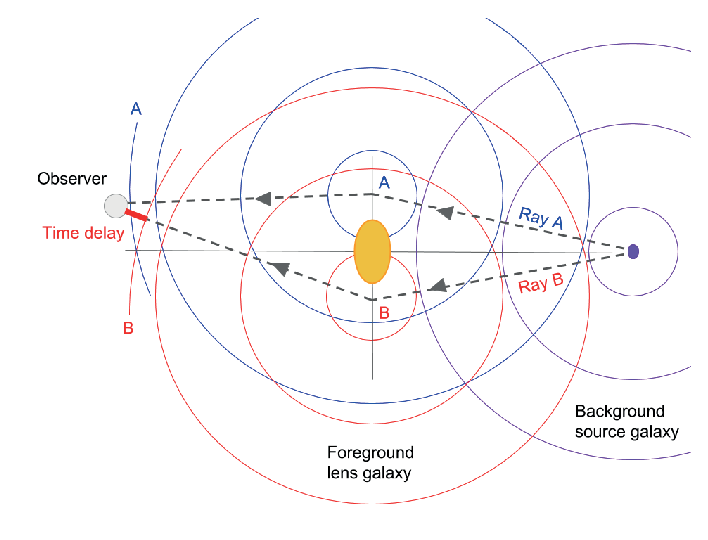
\includegraphics[width=0.80\textwidth]{pics/timedelayorigin.eps}
	\caption{Схематичная иллюстрация возникновения геометрического слагаемого в выражении для временной задержки (\cite{timedelaycosmography}).}
	\label{fig:timedelayorigin}
\end{figure} 

Непосредственно $\tau(\boldsymbol{\theta}, \boldsymbol{\beta})$ не поддаётся измерению. Но возможно измерить разницу этих величин для различных изображений:

\begin{equation}\label{eq:deltat}
\Delta \tau_{AB} = \tau(\boldsymbol{\theta}_A, \boldsymbol{\beta}) - \tau(\boldsymbol{\theta}_B, \boldsymbol{\beta}) = \frac{D_{\Delta t}}{c}  \Big( \Phi(\boldsymbol{\theta}_A, \boldsymbol{\beta}) - \Phi(\boldsymbol{\theta}_B, \boldsymbol{\beta}) \Big) = \frac{D_{\Delta t}}{c}  \Delta \Phi_{AB}.
\end{equation}

Нетрудно увидеть, что величина $D_{\Delta t}$, которая называется \textit{расстоянием временной задержки} (time-delay distance) и  определяется выражением (\ref{eq:dDt}), обратно пропорциональна $H_0$, что видно из формулы \eqref{eq:ang_dia_dist}. Важно также отметить множитель (1+$z_1$), который возникает из-за расширения Вселенной (временная задержка "происходит" \ на красном смещении $z_1$). Таким образом,

\begin{equation}\label{eq:dt}
\Delta \tau_{AB} \propto \frac{1}{H_0}\Delta \Phi_{AB}.
\end{equation}

%Knowledge of the lens mass distribution is of vital importance to the success of this cosmological inference: Equation 3 shows that the time delay distance is likely to be comparably sensitive to uncertainty in the predicted Fermat potential as it is to the measured time delay itself. More concentrated mass distributions with steeper density profiles produce longer time delays leading to shorter inferred time delay distances, and thus larger inferred values of H0 (Wucknitz, 2002; Kochanek, 2002; Suyu, 2012).

%Both α(θ) and ψ(θ) can be predicted given a model for the mass distribution of the lens.

Если смоделировать линзирующий потенциал $\Psi(\boldsymbol{\theta})$ и положение источника $\boldsymbol{\beta}$, которое может быть недоступным для наблюдений, и на основе этих данных рассчитать $\Delta \Phi_{AB}$, а также точно измерить временные задержки между изображениями, то можно вычислить значение постоянной Хаббла $H_0$ и других космологических параметров, например, безразмерных плотности материи $\Omega_m$ и тёмной энергии $\Omega_{\Lambda}$. Зависимость $D_{\Delta t}$ от $H_0$ наиболее сильная, поэтому дальнейшее исследование посвящено именно этому параметру.

Важно отметить, что распределение массы в линзы подвержено ряду вырождений, самым существенным из которых является так называемое "массовое вырождение слоя" \ (\textit{mass-sheet degeneracy}). Cуществует такое преобразование модели распределения массы в линзе, при котором наблюдаемые величины - положения изображений источника, относительные усиления, видимые звездные величины (наблюдаемый поток) - остаются прежними, в то время, как временные задержки могут испытывать серьёзные изменения (\cite{falco1985}). Для снятия данного вырождения необходимо привлечение дополнительной информации о потенциале линзы, которое может быть получено, например, моделированием динамики звёзд в галактике-линзе или изучением среды вдоль луча зрения (\cite{suyu2010}).

Особенности формирования изображений гравитационно-линзированных источников в зависимости от модели линзы подробно разобраны в литературе (\cite{blandfordnarayan1986}, \cite{kayserrefsdal1983}, \cite{narbart}, \cite{shwamb2002}).